%\documentclass[iop]{emulateapj}
\documentclass[preprint]{aastex}
%\documentclass[12pt, onecolumn]{emulateapj}
%\documentstyle[aas2pp4,natbib209]{article}

\usepackage{tikz}
\usepackage{natbib}
\usepackage{amsmath}

\usetikzlibrary{shapes.geometric, arrows}
\usetikzlibrary{fit}

\tikzstyle{hyper} = [circle, text centered, draw=black]%, fill=blue!30]
\tikzstyle{param} = [circle, text centered, draw=black]%, fill=green!30]
\tikzstyle{data} = [circle, text centered, draw=black, line width=2pt]%, 
fill=red!30]
%\tikzstyle{hyper} = [trapezium, trapezium left angle=70, trapezium right 
angle=110, minimum width=1cm, minimum height=0.5cm, text centered, draw=black, 
fill=green!30]
%\tikzstyle{param} = [rectangle, minimum width=1cm, minimum height=0.5cm, text 
centered, draw=black, fill=green!30]
%\tikzstyle{data} = [diamond, minimum width=1cm, minimum height=1cm, text 
centered, draw=black, fill=red!30]
%\tikzstyle{eqn} = [rectangle, minimum width=1cm, minimum height=0.5cm, text 
centered, draw=black]%, fill=green!30]
%\tikzstyle{latent} = [diamond, minimum width=1cm, minimum height=0.5cm, text 
centered, draw=black]%, fill=green!30]
\tikzstyle{arrow} = [thick,->,>=stealth]

\newcommand{\myemail}{aimalz@nyu.edu}
\newcommand{\textul}{\underline}

\shorttitle{A Probabilistic Approach to the Redshift Distribution Function}
\shortauthors{Malz and Hogg}

\begin{document}

\title{A Probabilistic Approach to the Redshift Distribution Function}

\author{A.I. Malz\altaffilmark{1}}
\altaffiltext{1}{CCPP}
\email{aimalz@nyu.edu}

\author{D.W. Hogg\altaffilmark{1}}
\altaffiltext{1}{CCPP}
\email{david.hogg@nyu.edu}

\begin{abstract}
Upcoming galaxy surveys aim to produce posterior probability distribution 
functions on photometric redshift (zPDFs) for each galaxy observed, but no one 
has yet clearly presented a mathematically valid method for how to use zPDFs to 
do inference on the physical parameters relevant to galaxy evolution, 
large-scale structure, and cosmology.  By considering a generative model for 
zPDFs, this paper presents a fully consistent technique for exploring a general 
one-point statistic of redshift from a set of zPDFs as an example of how such 
data products should be used.  The method herein developed is demonstrated and 
tested on the redshift distribution function $N(z)$ as an example of one such 
one-point statistic.
\end{abstract}

\keywords{photo-z}

\clearpage
\section{Introduction}
\label{sec:intro}

The era of precision cosmology, heralded by weak gravitational lensing 
tomography and baryon acoustic oscillation peak measurements, has been enabled 
by photometric estimation of redshifts previously accessible only by time- and 
resource-intensive spectroscopic confirmation.  However, photometric redshifts 
(photo-zs) are susceptible to a number of errors, particularly their inherent 
noisiness due to the coarseness of photometric filters, systematic errors 
introduced by observational techniques, and catastrophic errors in which 
galaxies of one type at one redshift are mistaken for galaxies of another type 
at a different redshift.  In addition to these limitations in accuracy, there 
is also the matter of precision; photo-zs are often reported with error bars 
derived without inclusion of all systematic errors, including the different 
selection effects between the magnitude-spaces of galaxies for which photo-zs 
are desired and galaxies with spectroscopically confirmed redshifts used to 
calibrate photo-z estimators.

Since their conception \citep{Baum1962}, much effort has been dedicated to 
improving photo-zs, though they are still most commonly obtained by a maximum 
likelihood estimator (MLE) based on libraries of galaxy spectral energy 
distribution (SED) templates with conservative approaches to error estimation.  
Recent work has focused on identifying and removing catastrophic outliers when 
using photo-zs for inference.  \citep{Gorecki2014}  Sophisticated Bayesian 
techniques and cutting-edge machine learning methods have been employed to 
improve precision \citep{Carliles2010} and accuracy \citep{Sadeh2015}. 

An alternative to point estimates of photo-zs is redshift probability 
distribution function (zPDF) estimation, in which the full posterior 
probability function of the redshift of a galaxy is produced rather than MLEs.  
\citep{Budavari2009}  This option is favorable because it contains more 
potentially useful information than a point estimate while addressing all the 
problems associated with point estimates discussed above.  For example, there 
is no need to identify and remove catastrophic outliers because their zPDFs 
would be automatically downweighted in inference.  zPDFs are not without their 
own weaknesses, the foremost of which are the computation time and storage 
space necessary to calculate and record zPDFs for large galaxy surveys.  
\citep{CarrascoKind2014}  The Bayesian prior used in such calculations may be 
based on either empirical training sets of spectroscopically confirmed galaxies 
but must nonetheless be made with great caution.

There is not yet consensus on the best way to obtain zPDFs, and many methods 
have been proposed and tested in the literature.  An extension of the BPZ 
method of \citet{Benitez2000} that produces full posteriors (as opposed to a 
selection of local maxima) from an SED template library has been employed.  
\citep{Hildebrandt2012, Kelly2014, Lopez-Sanjuan2015}  zPDFs have also been 
obtained by a variety of trustworthy data-driven approaches in the literature: 
$k$-nearest neighbor algorithms with \citep{Ball2008} and without 
\citep{Sheldon2012} inclusion of photometric measurement errors, neural 
networks \citep{Bonnett2015a}, self-organizing maps \citep{CarrascoKind2014a}, 
prediction tree and random forest classification techniques 
\citep{Carliles2010, CarrascoKind2013}.  

zPDFs have been produced by completed surveys \citep{Hildebrandt2012, 
Sheldon2012} and will be produced by upcoming surveys 
\citep{LSSTScienceCollaboration2009, CarrascoKind2014a}.  Though their 
potential to improve estimates of physical parameters is tremendous, full 
posteriors have seldom been used to infer physical parameters.  (Notable 
exceptions include \citet{Applegate2014}.)  Furthermore, no implementation of 
inference with zPDFs has been presented with a mathematically consistent 
methodology.  The goal of this paper is to clearly present and validate a 
technique for the use of zPDFs in inference.  For simplicity, we consider only 
one-point statistics relevant to cosmology, though future work will extend this 
technique to higher-order statistics.

The redshift distribution function $N(z)$ serves as an ideal statistic upon 
which to demonstrate such an approach, in large part because it has been the 
subject of inference using zPDFs before.  \citep{Sheldon2012, Kelly2014, 
Benjamin2013, Bonnett2015a, Viironen2015}  $N(z)$ for observed galaxies can be 
used to validate survey selection functions used in generation of realistic 
mock catalogs used for many purposes.  \citep{Norberg2002}  $N(z)$ is also 
trivially related to the comoving distance density function $n(\chi)$ 
\citep{Hogg1999}, which is necessary for calculations of weak lensing 
tomography that are directly used to probe cosmological parameters via the weak 
lensing shear power spectrum.  \citep{Masters2015}

\clearpage
\subsection*{Temporary Notes}

\begin{itemize}
\item \citet{Baum1962} first proposes the concept of photometric estimation of 
redshifts.
\item \citet{Benitez2000} presents the BPZ template-based method of obtaining 
photo-zs and publishes code that produces the top three MAP values of the full 
posterior.  
\item \citet{Hogg1999} reviews the definitions of several distance measures 
used in cosmology.
\item \citet{Norberg2002} calculates $N(z)$ (or is it $n(z)$?) for 2dFGRS 
galaxies and use it to validate the selection function they used to generate 
mock catalogs.
%\item \citet{Sheth2007} uses zPDFs
%\item \citet{Mandelbaum2008} uses zPDFs
%\item \citet{Lima2008} uses the stacking method
%\item \citet{Ball2008}
\item \citet{Budavari2009} is an extremely comprehensive review of photo-zs 
from Bayesian perspective that motivates the production of photo-z posterior 
distributions. They also produce photo-z posterior distributions for SDSS 
galaxies using KDE in magnitude space rather than a grid and stratified 
sampling of the training set in magnitude space to improve support in areas 
dense in the test set but sparse in the training set.
%\item \citet{VanBreukelen2009} uses zPDFs
%\item \citet{Myers2009} uses zPDFs
%\item \citet{LSSTScienceCollaboration2009}
%\item \citet{Carliles2010}
%\item \citet{Hogg2010}
\item \citet{Sheldon2012} obtains and publishes a catalog of photo-z posteriors 
for SDSS DR8 via a $k-$ nearest neighbors algorithm corrected by a factor of 
the redshift distribution function of a spectroscopically confirmed sub-sample. 
 They also calculate $N(z)$ using a stacking method.
\item \citet{Hildebrandt2012} obtains photo-z likelihoods via BPZ (minimally 
modifying its default prior) and publishes a catalog based on CFHTLenS 
photometry.  They also compare calculating N(z) via stacked photo-z probability 
distribution functions to a histogram of the MAP redshifts and conclude 
stacking is superior to using point estimates.
\item \citet{Kelly2014} obtains photo-z likelihoods via BPZ (with the same 
modification as \citet{Hildebrandt2012}) and does inference of WL shear with 
them.  They also stack the individual zPDFs to obtain $N(z)$.
%\item \citet{Foreman-Mackey2013}
\item \citet{Hogg2012} reviews Bayesian probability, including rectifying some 
common pitfalls.
\item \citet{Applegate2014} does inference on the WL shear estimator with 
photo-z likelihoods from \citet{Kelly2014}.  I believe something may be a 
little fishy in the math regarding likelihoods vs. posteriors.
\item \citet{Benjamin2013} calculates $N(z)$ for WL tomography by the stacking 
method.  They compare stacked photo-z probability distribution functions to a 
spectroscopically confirmed sample and a reweighting thereof.
\item \citet{Gorecki2014} presents a likelihood ratio test to identify and 
remove from inference catastrophic outliers in point-estimate photo-zs.
%\item \citet{Menard2013}
%\item \citet{CarrascoKind2013}
%\item \citet{Rhodes2013}
\item \citet{Bonnett2015a} obtains zPDFs via a neural network and stacks them 
to estimate $N(z)$.
%\item \citet{CarrascoKind2014a}
%\item \citet{CarrascoKind2014}
%\item \citet{Foreman-Mackey2014}
%\item \citet{Lopez-Sanjuan2015}
%\item \citet{Viironen2015}
\item \citet{Sadeh2015} develops code producing photo-z probability 
distribution functions, although likelihoods and posteriors are used 
interchangeably and only some of their methods give the interim prior.  There 
is a good review of papers presenting methods for generating photo-z 
probability distribution functions.
\item \citet{Bonnett2015} compares $N(z)$ found via several photo-z fitting 
methods, including the reduction of photo-z probability distribution functions 
to point estimates via the mean in order to recommend a method for the output 
of DES, without considering the full probability distribution functions as 
valuable data products.
\item \citet{Masters2015} uses self-organizing maps to obtain photometric 
redshift point estimates where template-based methods are inappropriate (for 
poorly characterized high redshift populations) and emphasizes the applications 
to $N(z)$ and weak lensing.
\item \citet{Marshall2015} outlines a hierarchical model for parameter 
estimation in the context of the halo occupation distribution.
\item \citet{Asorey2016}
\end{itemize}

\clearpage
\section{Method}
\label{sec:meth}

It is best to begin with a general description of the problem at hand.  Let us 
consider a survey of $J$ galaxies $j$, each with photometric data 
$\vec{d}_{j}$; thus the entire survey produces the ensemble of data 
$\{\vec{d}_{j}\}_{J}$.  Each galaxy $j$ has a redshift $z_{j}$ that we would 
like to learn; redshift is a parameter in this case.  The distribution of the 
ensemble of redshifts $\{z_{j}\}_{J}$ may be described by the hyperparameters 
defining the redshift distribution function $N(z)$ that would like to find.  
This situation may be considered to be a probabilistic generative model, 
illustrated by the directed acyclic graph of Fig. \ref{fig:flow}.  

\begin{figure}
\vspace{0.5cm}
\begin{center}
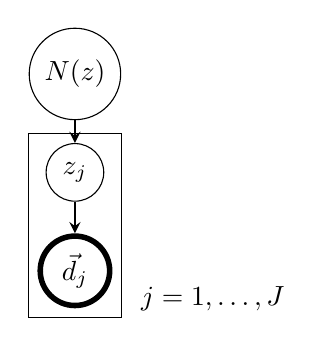
\begin{tikzpicture}[node distance=1cm]

\node (nz) [hyper] {$N(z)$};
\node (z) [param, below of=nz,yshift=-0.25cm] {$z_{j}$};
\node (mags) [data, below of=z,yshift=-0.25cm] {$\vec{d}_{j}$};
\node (survey) [draw=black,fit={(mags.west)(z.north)(mags.south)(mags.east)}] 
{};
\node [xshift=1.75cm,yshift=0.25cm] at (survey.south) {$j=1,\dots,J$};

\draw [arrow] (nz) -- (z);
\draw [arrow] (z) -- (mags);

\end{tikzpicture}
\caption{This directed acyclic graph illustrates a hierarchical model.}
\label{fig:flow}
\end{center}
\end{figure}

The redshift distribution function $N(z)$ shown in Eq. \ref{eq:distribution} 
gives the number of galaxies per unit redshift, effectively quantifying 
evolution in the number of galaxies.  \citep{Menard2013}  According to Eq. 
\ref{eq:density}, the redshift distribution function is related to the redshift 
density function $n(z)$, which gives the number of galaxies per unit redshift 
per unit volume.  The redshift density function provides additional information 
about cosmology via the rate of expansion over redshift.

\begin{eqnarray}
\label{eq:distribution}
N(z) &=& \frac{dN}{dz}
\end{eqnarray}

\begin{eqnarray}
\label{eq:density}
n(z) &=& \frac{dN}{dz\ d\Omega}
\end{eqnarray}

\clearpage
\subsection{Probabilistic Model}
\label{sec:prob}

We begin by parametrizing $N(z)$ in terms of $\vec{\theta}$, some set of 
parameters that define the form $N(z)$ may take in whatever basis we choose.  
At this point, these hyperparameters are quite general and may represent 
coefficients in a high-order polynomial as a function of redshift, a set of 
means and variances defining Gaussians that sum to the desired distribution, a 
set of histogram heights that describe a binned version of the redshift 
distribution function, etc.  We define a function $f_{\vec{\theta}}(z)=N(z)$ 
that transforms these hyperparameters into the redshift distribution function 
$N(z)$.  We shall denote the size of a given galaxy survey as $J$ galaxies 
labeled $j$.  The data in this case is a catalog of $J$ sets of photometry 
$\vec{d}_{j}$ as well as any associated errors on those measurements.  

In this paper, we shall work exclusively with log-probabilities.  What we wish 
to estimate is the full posterior probability of the parameters $\vec{\theta}$ 
given the data $\{\vec{d}_{j}\}_{J}$.  By Bayes' Rule, the full posterior may 
be expressed in terms of the full likelihood.

We will have to assume a hyperprior $\ln p(\vec{\theta})$ expressing our 
beliefs about the distribution of the hyperparameters.  This is a choice we 
cannot avoid making and one which is often inspired by the results of previous 
galaxy surveys.  We will, however, probe $\vec{\theta}$ with a quantity 
proportional to $p(\{\vec{d}_{j}\}_{J}$ because this quantity does not vary 
with the hyperparameters $\vec{\theta}$ and is generally unknowable.  The last 
term in this expression is the full likelihood 
$p(\{\vec{d}_{j}\}_{J}|\vec{\theta})$ of observing the data given the 
hyperparameters, which may be expanded in terms of a marginalization over the 
redshifts as parameters, as in Eq. \ref{eq:marginalize}.  

\begin{eqnarray}
\label{eq:marginalize}
\ln[p(\{\vec{d}_{j}\}_{J}|\vec{\theta})] &=& \ln\left[\int\ 
p(\{\vec{d}_{j}\}_{J}|\{z_{j}\}_{J})\ p(\{z_{j}\}_{J}|\vec{\theta})\ 
d\{z_{j}\}\right]
\end{eqnarray}

We shall make two assumptions of independence in order to make the problem 
tractable.  First, we take $\ln[p(\{\vec{d}_{j}\}_{J}|\{z_{j}\}_{J})]$ to be 
the sum of $J$ terms $\ln[p(\vec{d}_{j}|z_{j})]$, as in Eq. \ref{eq:indiedat}.  
This must not be true because of the properties of the survey shared among all 
observations.  We shall temporarily postpone discussion of the form of the 
individual likelihoods $p(\vec{d}_{j}|z_{j})$.  

\begin{eqnarray}
\label{eq:indiedat}
\ln[p(\{\vec{d}_{j}\}_{J}|\{z_{j}\}_{J})] &=& \sum_{j=1}^{J}\ 
\ln[p(\vec{d}_{j}|z_{j})]
\end{eqnarray}

Second, we shall assume the true redshifts $\{z_{j}\}_{J}$ are $J$ independent 
draws from the general $f_{\vec{\theta}}(z)$.  However, this assumption that 
the redshift of a galaxy $j$ is independent of the redshift of another galaxy 
$j'$ must be false because of the shared physical processes of the covariances 
of $N(z)$.  Additionally, $J$ itself is a Poisson random variable with expected 
value $J'$.  The combination of these is given by Eq. \ref{eq:indie}  It is 
important to note that $\int N(z)\ dz$ is not constrained to equal $J'$ but 
instead $J$, which can be thought of as another parameter.  A detailed 
discussion of this matter may be found in \citet{Foreman-Mackey2014}.

\begin{eqnarray}
\label{eq:indie}
\ln[p(\{z_{j}\}_{J}|\vec{\theta})] &=& -\int\ f_{\vec{\theta}}(z)\ dz +  
\sum_{j=1}^{J}\ \ln[p(z_{j}|\vec{\theta})]
\end{eqnarray}

%The redshift distribution function can be interpreted as being proportional to 
the likelihood that a random galaxy $j$ has a redshift $z_{j}=z$ where the 
constant of proportionality is the number $J$ of galaxies in the survey.  Thus 
the redshift distribution function we aim to estimate may be expressed in terms 
of the redshift parameter $z$ according to Eq. \ref{eq:params}.  

We may now combine terms into Eq. \ref{eq:posterior}.

\begin{eqnarray}
\label{eq:posterior}
\ln[p(\vec{\theta}|\{\vec{d}_{j}\}_{J})] &\propto& \ln[p(\vec{\theta})]\ -\int 
f_{\vec{\theta}}(z)\ dz + \sum_{j=1}^{J}\ \ln\left[\int\ p(\vec{d}_{j}|z_{j})\ 
p(z_{j}|\vec{\theta})\ dz_{j}\right]
\end{eqnarray}

Eq. \ref{eq:posterior} still contains the individual likelihoods 
$p(\vec{d}_{j}|z_{j})$ unaddressed since Eq. \ref{eq:marginalize} that are this 
case is inaccessible; it is worth discussing why this is the case.  Both 
empirical and data-driven methods for obtaining zPDFs effectively assign to 
each galaxy's photometry $\vec{d}_{j}$ both a redshift $z_{j}$ and some 
nuisance parameters contained in $\vec{\theta}^{0}$ related to the generative 
model for photometry from redshifts, encapsulated by 
$p(z_{j}|\vec{d}_{j},\vec{\theta}^{0})$.  These may include some parameters 
defining intrinsic galaxy spectra and instrumental effects, for example. (See 
\citet{Benitez2000} for more detail.)  In the case of estimating $N(z)$ 
photometrically it is common to use $\vec{\theta}^{0}$ corresponding to $N(z)$ 
derived from some different, spectroscopically confirmed sample or from a 
cosmological simulation.  For statistical purposes, we would like any interim 
prior to be uninformative, but this is rarely achievable.

%If we were to attempt to calculate likelihoods 
$p(\vec{d}_{j}|z_{j},\vec{\theta}^{0})$, we would be unable to integrate out 
these nuisance parameters.  (See \citet{Hogg2012} for a comprehensive 
presentation of the mathematics behind why this is the case.)  However, 
posteriors $p(z_{j},\vec{\theta}^{0}|\vec{d}_{j})$ could be transformed to 
zPDFs $p(z_{j}|\vec{d}_{j},\vec{\theta}^{0})$ by integrating 
$p(z_{j},\vec{\theta}^{0}|\vec{d}_{j})\ p(\vec{\theta}^{0})$ with respect to 
$\vec{\theta}^{0}$, given the prior  $p(\vec{\theta}^{0})$ of those parameters. 
 

Instead, we would like to work with posteriors rather than likelihoods in Eq. 
\ref{eq:marginalize}.  The method outlined here is valid regardless of how the 
zPDF $p(z_{j}|\vec{d}_{j},\vec{\theta}^{0})$ is calculated so the approach to 
producing zPDFs will not be discussed; though the matter is outside the scope 
of this paper, various methods have been presented in the literature. 
\citep{Sheldon2012, Ball2008, CarrascoKind2013, CarrascoKind2014a}  However, we 
will need an explicit statement of this interim prior $\vec{\theta}^{0}$ for 
whatever method is chosen to produce zPDFs.  To perform the necessary 
transformation from likelihoods to posteriors, we follow the reasoning of 
\citet{Marshall2015}.  Let us consider the probability of the parameters 
$z_{j}$ conditioned on the data $\vec{d}_{j}$ and an interim prior 
$\vec{\theta}^{0}$ and rewrite the problematic likelihood of Eq. 
\ref{eq:posterior} as Eq. \ref{eq:trick}.  

\begin{eqnarray}
\label{eq:trick}
p(\vec{d}_{j}|z_{j}) &=& p(\vec{d}_{j}|z_{j})\ 
\frac{p(z_{j}|\vec{d}_{j},\vec{\theta}^{0})}{p(z_{j}|\vec{d}_{j},\vec{\theta}^{0
})}
%p(\vec{\theta}|\{\vec{d}_{j}\}_{J}) &=& 
\frac{p(\vec{\theta})}{p(\{\vec{d}_{j}\}_{J})}\exp[-\int N(z)\ 
dz]\prod_{j=1}^{J}\int\ p(\vec{d}_{j}|z_{j})\ p(z_{j}|\vec{\theta})\ 
\frac{p(z_{j}|\vec{d}_{j},\vec{\theta}^{0})}{p(z_{j}|\vec{d}_{j},\vec{\theta}^{0
})}\ dz_{j}
\end{eqnarray}

Once the interim prior $\vec{\theta}^{0}$ is explicitly introduced, we may 
expand the denominator according to Eq. \ref{eq:bayes} to get Eq. 
\ref{eq:expand}.  We again expand the term 
$p(\vec{d}_{j}|z_{j},\vec{\theta}^{0})$ to obtain Eq. \ref{eq:indterm}.  
Canceling the undesirable likelihood terms $p(\vec{d}_{j}|z_{j})$ and 
$p(\vec{d}_{j}|\vec{\theta}^{0})$ yields Eq. \ref{eq:cancel}.  We put this all 
together to get the full posterior Eq. \ref{eq:final}.

\begin{eqnarray}
\label{eq:expand}
p(\vec{d}_{j}|z_{j}) &=& p(\vec{d}_{j}|z_{j})\ 
p(z_{j}|\vec{d}_{j},\vec{\theta}^{0})\ 
\frac{p(\vec{d}_{j}|\vec{\theta}^{0})}{p(z_{j}|\vec{\theta}^{0})\ 
p(\vec{d}_{j}|z_{j},\vec{\theta}^{0})}
%p(\vec{\theta}|\{\vec{d}_{j}\}_{J}) &=& 
\frac{p(\vec{\theta})}{p(\{\vec{d}_{j}\}_{J})}\exp[-\int N(z)\ 
dz]\prod_{j=1}^{J}\int\ p(\vec{d}_{j}|z_{j})\ p(z_{j}|\vec{\theta})\ 
p(z_{j}|\vec{d}_{j},\vec{\theta}^{0})\ 
\frac{p(\vec{d}_{j}|\vec{\theta}^{0})}{p(\vec{d}_{j}|z_{j},\vec{\theta}^{0})\ 
p(z_{j}|\vec{\theta}^{0})}\ dz_{j}
\end{eqnarray}

\begin{eqnarray}
\label{eq:indterm}
p(\vec{d}_{j}|z_{j}) &=& p(\vec{d}_{j}|z_{j})\ 
p(z_{j}|\vec{d}_{j},\vec{\theta}^{0})\ 
\frac{p(\vec{d}_{j}|\vec{\theta}^{0})}{p(z_{j}|\vec{\theta}^{0})\ 
p(\vec{d}_{j}|z_{j})\ p(\vec{d}_{j}|\vec{\theta}^{0})}
%p(\vec{\theta}|\{\vec{d}_{j}\}_{J}) &=& 
\frac{p(\vec{\theta})}{p(\{\vec{d}_{j}\}_{J})}\exp[-\int N(z)\ 
dz]\prod_{j=1}^{J}\ \int\ p(z_{j}|\vec{d}_{j},\vec{\theta}^{0})\ 
\frac{p(z_{j}|\vec{\theta})}{p(z_{j}|\vec{\theta}^{0})}\ dz_{j}
\end{eqnarray}

\begin{eqnarray}
\label{eq:cancel}
p(\vec{d}_{j}|z_{j}) &=& 
\frac{p(z_{j}|\vec{d}_{j},\vec{\theta}^{0})}{p(z_{j}|\vec{\theta}^{0})}
%p(\vec{\theta}|\{\vec{d}_{j}\}_{J}) &=& 
\frac{p(\vec{\theta})}{p(\{\vec{d}_{j}\}_{J})}\exp[-\int N(z)\ 
dz]\prod_{j=1}^{J}\ \int\ p(z_{j}|\vec{d}_{j},\vec{\theta}^{0})\ 
\frac{p(z_{j}|\vec{\theta})}{p(z_{j}|\vec{\theta}^{0})}\ dz_{j}
\end{eqnarray}

\begin{eqnarray}
\label{eq:final}
%p(\vec{\theta}|\{\vec{d}_{j}\}_{J}) &=& 
\frac{p(\vec{\theta})}{p(\{\vec{d}_{j}\}_{J})}\exp[-\int N(z)\ 
dz]\prod_{j=1}^{J}\ \int\ p(z_{j}|\vec{d}_{j},\vec{\theta}^{0})\ 
\frac{p(z_{j}|\vec{\theta})}{p(z_{j}|\vec{\theta}^{0})}\ dz_{j}
\ln[p(\vec{\theta}|\{\vec{d}_{j}\}_{J})] &\propto& \ln[p(\vec{\theta})]-\int 
f_{\vec{\theta}}(z)\ dz + \sum_{j=1}^{J}\ \ln\left[\int\ 
p(z_{j}|\vec{d}_{j},\vec{\theta}^{0})\ 
\frac{p(z_{j}|\vec{\theta})}{p(z_{j}|\vec{\theta}^{0})}\ dz_{j}\right]
\end{eqnarray}

The argument of the integral in the posterior of Eq. \ref{eq:final} depends 
solely on knowable quantities (and those we must assume) and can be calculated 
for a given set of zPDFs $\{p(z_{j}|\vec{d}_{j},\vec{\theta}^{0})\}_{J}$ and 
the interim prior $\vec{\theta}^{0}$ upon which their determination was based, 
noting the relation of Eq. \ref{eq:params}.  Since we cannot know 
$p(\{\vec{d}_{j}\}_{J})$, we sample the desired distribution 
$p(\vec{\theta}|\{\vec{d}_{j}\}_{J})$ using Monte Carlo-Markov chain (MCMC) 
methods.  

\begin{eqnarray}
\label{eq:params}
p(z_{j}|\vec{\theta}) &=& \frac{f_{\vec{\theta}}(z_{j})}{\int\ 
f_{\vec{\theta}}(z_{j})\ dz_{j}}
\end{eqnarray}

To be clear, the following assumptions must be made in order to apply this 
method:

\begin{enumerate}
\item Photometric measurements of galaxies are independent Poisson draws from 
the set of all galaxies such that Eqs. \ref{eq:indiedat} and \ref{eq:indie} 
hold.
\item We take the individual galaxy zPDFs to be accurate estimates of the 
posteriors $\{p(z_{j}|\vec{d}_{j})\}_{J}$ and assume we are given the interim 
prior $\vec{\theta}^{0}$ used to produce them.
\item One must assume a hyperprior $p(\vec{\theta})$ constraining the 
underlying probability of the variables defining the hyperparameters 
$\vec{\theta}$.
\end{enumerate}

These assumptions have known limitations.  First, the observations 
$\{\vec{d}_{j}\}_{J}$ are not a set of independent measurements; they are 
correlated not only by the conditions of the experiment under which they were 
made but also by $N(z)$ and other physical processes governing underlying 
galaxy spectra.  Second, the zPDFs 
$\{p(z_{j}|\vec{d}_{j},\vec{\theta}^{0})_{J}$ may not be trustworthy; there is 
not yet agreement on the best technique to obtain zPDFs, and the interim prior 
$\vec{\theta}^{0}$ may not be appropriate or even known to us as consumers of 
zPDFs.  Third, the hyperprior $p(\vec{\theta})$ may be quite arbitrary; it may 
be poorly motivated if the underlying physics is complex.

\clearpage
\subsection{Competing Methods}
\label{sec:sheldon}

It will be desirable to compare the result of this method to what would have 
been obtained by two popular alternatives used in the literature.   

The first, hereafter referred to as stacking, directly calculates the posterior 
for the entire dataset using the posteriors for each galaxy according to Eq. 
\ref{eq:stack}.  \citep{Lima2008}  It must be noted here that Eq. 
\ref{eq:stack} is not mathematically valid.  (See \citet{Hogg2012} for 
details.)  

\begin{eqnarray}
\label{eq:stack}
\exp[\theta_{k}]\Delta_{k} &=& \sum_{j=1}^{J}\ 
p(B_{k}|\vec{d}_{j},\vec{\theta}^{0})
\end{eqnarray}

The second, hereafter referred to as point estimation, converts the individual 
galaxy posteriors $p(B_{k}|\vec{d}_{j},\vec{\theta}^{0})$ into delta functions 
at the redshift bin of maximum posterior (MAP) probability according to Eq. 
\ref{eq:map}, or at the redshift bin corresponding to the expected value 
($E[z]$) of Eq. \ref{eq:expval}, before applying Eq. \ref{eq:stack}.  The 
result is a histogram of interim MAP or $E[z]$ redshift point estimates.

\begin{eqnarray}
\label{eq:map}
p(B_{k}|\vec{d}_{j},\vec{\theta}^{0}) &=& 
\left\{\begin{array}{cc}1&argmax_{k}(p(B_{k}|\vec{d}_{j},\vec{\theta}^{0}))\\0&e
lse\end{array}\right\}
\end{eqnarray}

\begin{eqnarray}
\label{eq:expval}
p(B_{k}|\vec{d}_{j},\vec{\theta}^{0}) &=& 
\left\{\begin{array}{cc}1&\int_{0}^{K} \bar{z}_{k}\ 
p(B_{k}|\vec{d}_{j},\vec{\theta}^{0}) dk\\0&else\end{array}\right\}
\end{eqnarray}

These two approaches have been compared to one another by 
\citet{Hildebrandt2012} and \citet{Benjamin2013}.

\clearpage
\section{Experiments}
\label{sec:exp}

We ran several tests of this approach to demonstrate its validity and usage 
using a procedure outlined in this section.  In Sec. \ref{sec:mock} we describe 
the method by which sets of simulated zPDFs $\{p(z_{j}|\vec{d}_{j})\}_{J}$ are 
generated in all test cases.  In Sec. \ref{sec:mcmc} we describe the algorithm 
used to compute the full posterior distribution 
$p(\vec{\theta}|\{\vec{d}_{j}\}_{J})$.  In Sec. \ref{sec:diag} we outline the 
measures used to evaluate the performance of the method, including the 
competing methods with which our results will be compared.  Then in Sec. 
\ref{sec:valid} we motivate and present the results of several informative 
tests.

\clearpage
\subsection{Mock data}
\label{sec:mock}

To generate mock photometric redshift posteriors, we first produce a catalog of 
true redshifts.  We choose a physically-motivated $p^{0}(z)$ defining the 
general shape of $N(z)$ over a specified redshift range $[z_{min},z_{max}]$.  
Here we shall set it to a weighted sum of truncated Gaussians chosen to impose 
recognizably recoverable features on the true $N(z)$.  The true survey size $J$ 
is a Poisson random variable distributed about a target survey size of $J'$.  
Next we take $J$ samples of $z\sim p^{0}(z)$ to obtain the true redshift 
catalog $\{z_{j}^{0}\}_{J}$.  

The catalog of redshift posteriors $\{p(z_{j}|\vec{d}_{j})\}_{J}$ is chosen to 
be a set of Gaussian distributions, truncated to the redshift range of $N(z)$, 
because it is the simplest extension of the standard redshift point estimates 
with reported error bars.  To simulate the fact that inaccuracy increases with 
redshift, each Gaussian is centered at a redshift $z_{j}'$ separated from the 
true redshift $z_{j}^{0}$ by a Gaussian random variable $\epsilon_{j}$ selected 
from a distribution of mean of 0 and variance $v_{j}\propto(1+z_{j}^{0})^{2}$.  
To simulate the fact that imprecision also increases with redshift, the 
variances of the truncated Gaussian redshift posteriors are also set to 
$\{v_{j}\}_{J}$.

Before constructing the redshift posterior catalog, we must choose the interim 
prior $\vec{\theta}^{0}$ introduced in Eq. \ref{eq:trick} that encodes our 
beliefs about the way data is produced.  By default we choose a flat 
distribution. We impose a binning $B_{k}=[z^{B}_{k-1},z^{B}_{k}]$ on the 
redshift range from $z^{B}_{0}=z_{min}$ to $z^{B}_{K}=z_{max}$ with bin widths 
$\Delta_{k}\equiv z_{k}-z_{k-1}$.  To obtain the desired interim redshift 
posteriors, we simply normalize the integral of the product of the interim 
prior and the Gaussian redshift posterior over the bins.  

A random sampling of such interim redshift posteriors with $K=???$ is shown in 
Fig. \ref{fig:nullpzs}.

\begin{figure}
%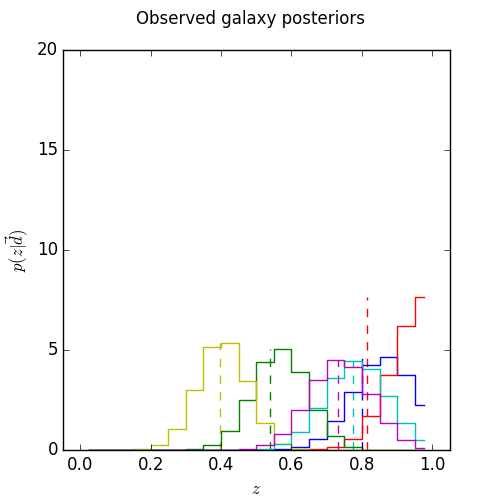
\includegraphics[width=0.5\textwidth]{null/samplepzs.png}
\caption{}
\label{fig:nullpzs}
\end{figure}

\clearpage
\subsection{Data}
\label{sec:data}

We also test this method on a random subset of the published redshift 
posteriors of SDSS III DR 10.  A random sampling of the provided redshift 
posteriors of dimension $K=35$ for $z_{min}=0.3$ and $z_{max}=1.4$ is shown in 
Fig. \ref{fig:datapzs}.  The interim prior used for this set of interim 
redshift posteriors is calculated using the method of \citet{Sheldon2012} and 
was reproduced here since the final result was not published elsewhere.

\begin{figure}
%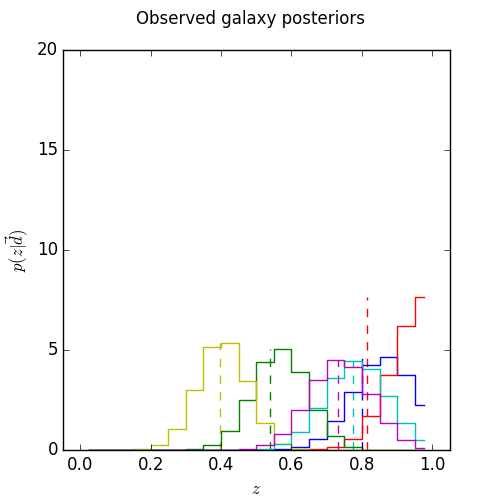
\includegraphics[width=0.5\textwidth]{null/samplepzs.png}
\caption{}
\label{fig:datapzs}
\end{figure}

\clearpage
\subsection{Implementation}
\label{sec:mcmc}

The testing procedure is implemented in \texttt{Python}.  The code takes as 
input a \texttt{csv} file containing the basis for the parametrization of 
redshift space, a specification of the interim prior $\vec{\theta}^{0}$, and a 
catalog of $J$ zPDFs $\{p(B_{j}|\vec{d}_{j},\vec{\theta}^{0})\}_{J}$ each of 
length $K$ in the given basis.  The assumed prior distribution is described in 
Sec. \ref{sec:prior}.

The \texttt{emcee} implementation of the Metropolis-Hastings algorithm is 
applied to sample the full posterior of Eq. \ref{eq:logpost}.   
\citep{Foreman-Mackey2013}   The sampler is initialized with $W=2K$ walkers 
each with a value chosen from a Gaussian distribution of identity covariance 
around a sample from the prior distribution.  At each iteration $i$, a proposal 
distribution $\vec{\theta}^{i}$ generated from this prior distribution and 
evaluated for acceptance to or rejection from the desired posterior 
distribution according to the algorithm outlined below.  

\begin{enumerate}
\item \label{it:randsamp} Randomly sample the prior $p(\vec{\theta})$ to 
generate a proposal $\vec{\theta}^{i}$.
\item Calculate the log pseudo-posterior as in Eq. \ref{eq:logpost} to produce 
$\ln\tilde{p}(\vec{\theta}^{i}|\{\vec{d}_{j}\}_{J})$.
\item Calculate 
$a=\ln\tilde{p}(\vec{\theta}^{i}|\{\vec{d}_{j}\}_{J})-\ln\tilde{p}(\vec{\theta}|
\{\vec{d}_{j}\}_{J})$.
\item If $a\geq0$, set and record $\vec{\theta}=\vec{\theta}^{i}$.\\
If $a<0$, select a random number $n$ from the uniform distribution between 0 
and 1.
\begin{enumerate}
\item If $n<\exp[a]$, set and record $\vec{\theta}=\vec{\theta}^{i}$.
\end{enumerate}
\item Check if the threshold condition has been achieved; if not, return to 
Step \ref{it:randsamp}.
\end{enumerate}

Here, the threshold condition is defined in terms of sub-runs of $I_{0}$ 
accepted samples.  When the variance of the log probabilities is less than the 
change in median log probability over the sub-run, the burn-in period is 
considered complete.  When this occurs, an additional number of sub-runs equal 
to the number $I'$ of sub-runs consumed by the burn-in period are completed 
such that the total number of accepted samples is $I=2I'$.  

The input/output format chosen for this work is \texttt{HDF5} because of its 
efficiency for large amounts of data.  The resulting output is a set of $I$ 
ordered \texttt{hickle} files (should I use \texttt{FITS}?) enumerated by 
$\rho$ containing the state information after each sub-run.  The state 
information includes $\frac{I_{0}}{t}$ actual samples $\vec{\theta}^{i}$ for a 
pre-specified chain thinning factor and their full posterior probabilities 
$p(\vec{\theta}^{i}|\{\vec{d}_{j}\}_{J})$ as well as the autocorrelation times 
and acceptance fractions calculated for each element of $\vec{\theta}$ over the 
entire sub-run.  These two summary statistics are described in Sec. 
\ref{sec:diag}, along with the proper use of the other outputs in interpreting 
the results of the code.

\clearpage
\subsubsection{Prior}
\label{sec:prior}

The method of Sec. \ref{sec:mcmc} involves the assumption of a prior 
distribution on the hyperparameters in $\vec{\theta}$.  The prior chosen here 
is a multivariate normal distribution with mean $\vec{\theta}^{0}$ equal to the 
interim prior and covariance $\textul{\Sigma}$ inspired by one used in Gaussian 
processes, given by Eq. \ref{eq:priorcov}.  This choice is made to permit draws 
from this prior distribution to produce shapes similar to that of the true 
$\tilde{\theta}$.  Here, the parameters of this covariance matrix are set to 
the small numbers $q=?$, $e=?$, and $t=?$.  We adapt the full posterior of Eq. 
\ref{eq:final} to the binning of redshift space chosen in Sec. \ref{sec:mock}.

\begin{eqnarray}
\label{eq:priorcov}
\Sigma_{a,b} &=& q\ \exp[-\frac{e}{2}\ (\bar{z}_{a}-\bar{z}_{b})^{2}]\ +\ t\ 
v_{a,b}
\end{eqnarray}

The implementation of MCMC is initialized with $2K$ walkers taking values from 
a Gaussian ball around a sample from the prior distribution.  Such samples from 
the prior are shown in Fig. \ref{fig:nullprior} for $K=???$.

\begin{figure}
%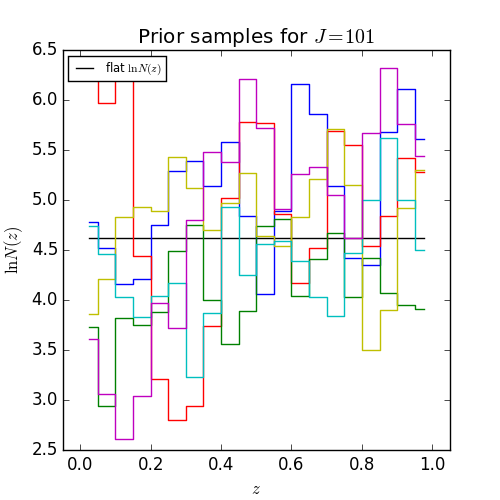
\includegraphics[width=0.5\textwidth]{null/priorsamps.png}
\caption{}
\label{fig:nullprior}
\end{figure}

\clearpage
\subsection{Diagnostics}
\label{sec:diag}

The results of the computation described in Sec. \ref{sec:mcmc} are evaluated 
on the basis of several diagnostics measures, briefly described below.  See 
\citet{Foreman-Mackey2013} for a more complete exploration of the metrics 
discussed in Sec. \ref{sec:acorr}.  The tests conducted here are also compared 
to the results one would obtain from alternative methods found in the 
literature, outlined in \ref{sec:sheldon}.

\clearpage
\subsubsection{Autocorrelation Time}
\label{sec:acorr}

The autocorrelation time is effectively a measure of the convergence rate of 
the method and can be described as the expected number of iterations necessary 
to accept a sample independent of the current sample.  A sampler that converges 
faster will have a smaller autocorrelation time, and smaller autocorrelation 
times are preferable because it means fewer iterations are wasted on 
non-independent samples when independent samples are desired.  Typically, the 
autocorrelation time decreases with successive iterations through a burn-in 
phase before leveling out.

\clearpage
\subsubsection{Posterior Probability Evolution}
\label{sec:probs}

In order to evaluate the duration of the burn-in phase, it can be helpful to 
examine the evolution of the posterior probability of each accepted set of 
parameters.  Though the probability associated with the initial values will 
likely be quite low, the probability should improve for subsequent accepted 
parameter values.  As with the diagnostics of Secs. \ref{sec:acorr} and 
\ref{sec:afrac}, the posterior probability of samples will asymptotically 
approach some more favorable value with more iterations.  The burn-in phase may 
be identified as the number of iterations necessary before the probabilities 
are sufficiently close to the value at which they level out.  Samples accepted 
during the burn-in phase are typically discounted from analysis.  

The posterior probabilities for the samples may also be compared to the 
posterior obtained by the competing approaches discussed in Sec. 
\ref{sec:sheldon}; higher posterior probabilities indicate a better fit than 
the alternative.  The distribution of the posterior probabilities of the 
samples may also be an informative measure of performance.

\clearpage
\subsubsection{Parameter Evolution}
\label{sec:params}

An intuitive diagnostic used here is the evolution of the parameter values 
themselves.  We would like to see each walker move throughout parameter space 
near the true value rather than remaining stationary or in some small region 
around another value.  We can visually inspect the parameter values each walker 
takes over successive iterations to ensure that the walkers are not being 
caught in small regions of parameter space far from the true parameter values.  

Inspection of the parameter evolution can also be a good test of the 
appropriateness of the prior distribution; if the covariance matrix of the 
prior distribution is too restrictive, the walkers will not be able to sample 
parameter values far from their initialization.  

\clearpage
\subsubsection{Parameter Values}
\label{sec:samps}

Sampled values of the vector of parameters are also visually inspected for 
goodness of fit to the truth.  When using simulated data where a true value is 
known, the sampler is performing well if samples are near the true value.  The 
distribution of the parameter values can also reveal how well the samples fit 
the data.  If there is a strongly peaked distribution of values for a 
parameter, it ought to peak close to the true value if we are to conclude that 
the sampler is successful; if the distribution is broad, it may reflect 
inherent uncertainty in inferring the parameters.  We shall consider the kernel 
density estimate (KDE) of each element of the parameter vector.

\clearpage
\subsubsection{Summary Statistics}
\label{sec:stats}

Beyond visual inspection of samples, we calculate summary statistics to 
quantitatively compare different estimators' ability to recover the truth.  
Three measures of accuracy of parameter samples $\vec{\theta}^{i}$  have been 
considered here.  

The likelihood ratio comparing the sampler to competing methods may be 
calculated for a sample $\vec{\theta}^{i}$ as in Eq. \ref{eq:llr}.  Values of 
$A$ greater than 0 indicate the sampler fits the data better than the competing 
method.  The log posterior probabilities of Sec. \ref{sec:probs} are used to 
obtain the log likelihoods via Eq. \ref{eq:logpost} and the sample values 
themselves are used to calculate the prior probability term according to Eq. 
\ref{eq:llr-how}; the difference between the log posteriors and the log prior 
probability is the log likelihood, and the difference between log likelihoods 
is the log likelihood ratio.  Because the sampler produces many samples of 
parameter values, the log likelihood ratio for the sampler versus each 
alternative is a distribution of values.

\begin{eqnarray}
\label{eq:llr}
A(\vec{\theta}^{i}) &=& 
-2\ln[\tilde{p}(\{\vec{d}_{j}\}_{J}|\vec{\theta}_{test})]+2\ln[\tilde{p}(\{\vec{
d}_{j}\}_{J}|\vec{\theta}^{i})]
\end{eqnarray}

\begin{eqnarray}
\label{eq:llr-how}
\ln[\tilde{p}(\{\vec{d}_{j}\}_{J}|\vec{\theta})] &=& 
\ln[\tilde{p}(\vec{\theta}|\{\vec{d}_{j}\}_{J})]-\ln[p(\vec{\theta})]
\end{eqnarray}

In simulated cases where the true parameter values are known, we also calculate 
the Kullback-Leibler divergence (KLD), given in Eq. \ref{eq:kl} which measures 
a distance between parameter values $\vec{\theta}^{a}$ and $\vec{\theta}^{b}$ 
that is invariant under changes of variables.  We note that $KL_{ab}\neq 
KL_{ba}$, so both must be calculated.  In simulated tests, one of 
$\vec{\theta}^{a}$ and $\vec{\theta}^{b}$ are the true value and the other is 
the value produced by one of the methods in question.  For the sampler, the KLD 
is calculated for all samples and shown as a distribution of KLD values.

\begin{eqnarray}
\label{eq:kl}
KL_{ab} &=& \sum_{k=1}^{K}\ \exp[\theta_{k}^{a}]\ 
\ln\left[\frac{\theta_{k}^{a}}{\theta_{k}^{b}}\right]\ \Delta_{k}
\end{eqnarray}

The mean squared error of samples relative to the true value may also be 
calculated.  Both the variance $\sigma^{2}$ and $\chi^{2}$ statistics are 
calculated for the accepted samples and for the competing methods relative to 
the true value in the simulated tests.

\clearpage
\subsubsection{Marginalized Maximum Likelihood}
\label{sec:mmle}

The method outlined in Sec. \ref{sec:mcmc} is predicted to produce samples that 
approach the marginalized maximum likelihood estimator.  The marginalized 
likelihood (MML) is the last two terms of Eq. \ref{eq:logpost}, isolated in Eq. 
\ref{eq:mmle}.  This quantity is maximized to give the maximum marginalized 
likelihood estimator (MMLE) of $\vec{\theta}$.  For some scientific purposes, 
this quantity is a sufficient estimator of $\vec{\theta}$.  However, it is 
often valuable to learn the posterior distribution of the components of 
$\vec{\theta}$, which are not produced by the MMLE alone and can only be 
obtained by the sampling method of this paper.

\begin{eqnarray}
\label{eq:mmle}
\ln[\tilde{p}(\{\vec{d}_{j}\}_{J}|\vec{\theta})] = 
-\sum_{k=1}^{K}\exp[\theta_{k}]\Delta_{k}+\sum_{j=1}^{J}\ln\left[\sum_{k=1}^{K}\
exp\left[\ln[p(B_{k}|\vec{d}_{j},\vec{\theta}^{0})]+\theta_{k}-\theta_{k}^{0}+\l
n[\Delta_{k}]\right]\right]
\end{eqnarray}

The \texttt{fmin} minimizer provided by \texttt{scipy.optimize} is used to find 
the MMLE.  We check that the MML is truly maximized by comparing its MML to 
those of weighted averages of the MMLE and the true parameter values in 
simulated cases.

\clearpage
\section{Validation Tests}
\label{sec:valid}

The code was tested on several simulated datasets.  The fiducial experiment of 
Sec. \ref{sec:null} was generated by code following the procedure given in Sec. 
\ref{sec:mock}.  Four other cases varied the shapes of the zPDFs (Secs. 
\ref{sec:noisy} and \ref{sec:multi}), the underlying $N(z)$ (Sec. 
\ref{sec:fake}), and the interim prior $\vec{\theta}^{0}$ (Sec. 
\ref{sec:badprior}).  

\clearpage
\subsection{Fiducial Case}
\label{sec:null}

For the fiducial experiment, we precisely follow the procedure outlined in Sec. 
\ref{sec:mock} to simulate data.  In this example $K=?$ and $J=?$.  Fig. 
\ref{fig:nulltrueNz} shows the true value of $N(z)$ for this case.  Fig. 
\ref{fig:nullcat} shows the MAP and $E[z]$ redshifts along with the zPDF 
magnitudes as a function of the true redshifts.  We precisely follow the 
procedure of Sec. \ref{sec:mcmc} for the computation.  

%\begin{figure}
%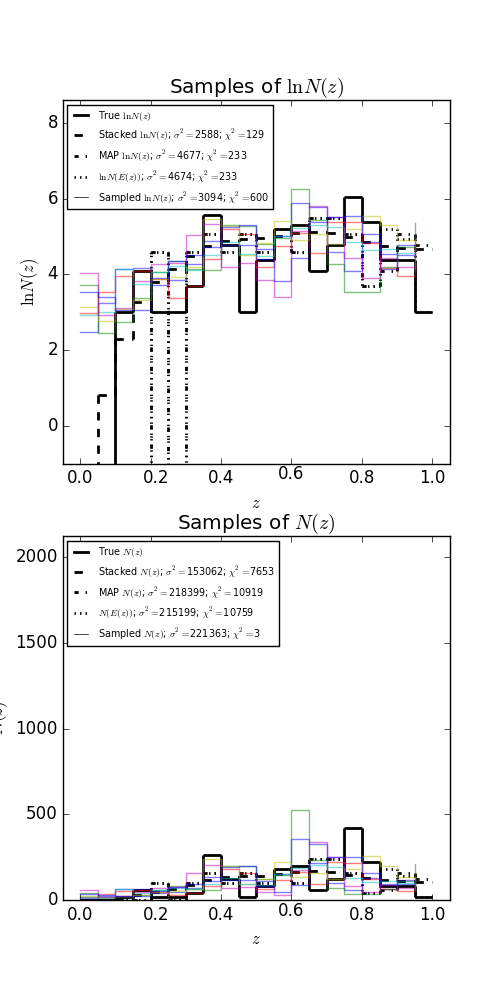
\includegraphics[width=0.5\textwidth]{null/samps.png}
%\caption{}
%\label{fig:nullparam}
%\end{figure}

\clearpage
\subsection{Noisy zPDFs}
\label{sec:noisy}

In this test, we aim to simulate more realistic zPDFs by modifying the 
procedure of Sec. \ref{sec:mock} to introduce imprecision that increases 
noisily with true redshift.  Several factors contribute to photometric 
redshifts' increased uncertainty with redshift.  As redshift increases, so do 
photometric errors.  There is a greater risk of encountering unknown SEDs at 
higher redshift where fewer spectroscopic explorations have been conducted.  

We introduce one change in the steps of Sec. \ref{sec:mock}.  After the shifted 
redshifts $z'_{j}$ are chosen, the variance of the Gaussian describing the 
shape of the zPDF is chosen to not be the same $v_{j}$ but rather a random 
variable $v_{j}'$ drawn from a Gaussian of mean $v_{j}$ and variance 
$v_{j}^{2}$.  Some interim redshift posteriors from such a test are shown in 
Fig. \ref{fig:noisypzs} for $K=???$.  The rest of the steps in Sec. 
\ref{sec:mcmc} are then followed precisely.

\begin{figure}
%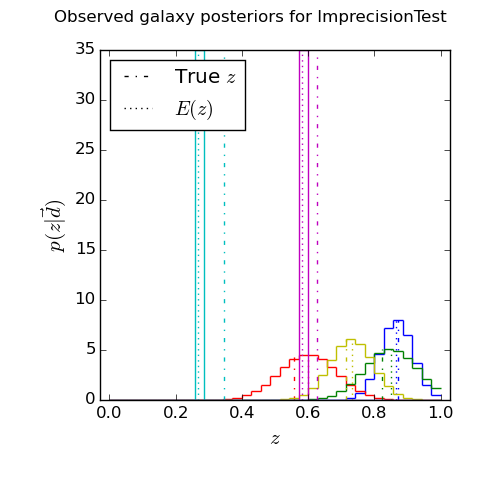
\includegraphics[width=0.5\textwidth]{sigma/samplepzs.png}
\caption{Unimodal, noisy zPDFs are used in this test.  Noise is introduced in 
the form of variances that are Gaussian random variables rather than fixed 
values tied to the true redshift.}
\label{fig:noisypzs}
\end{figure}

%\begin{figure}
%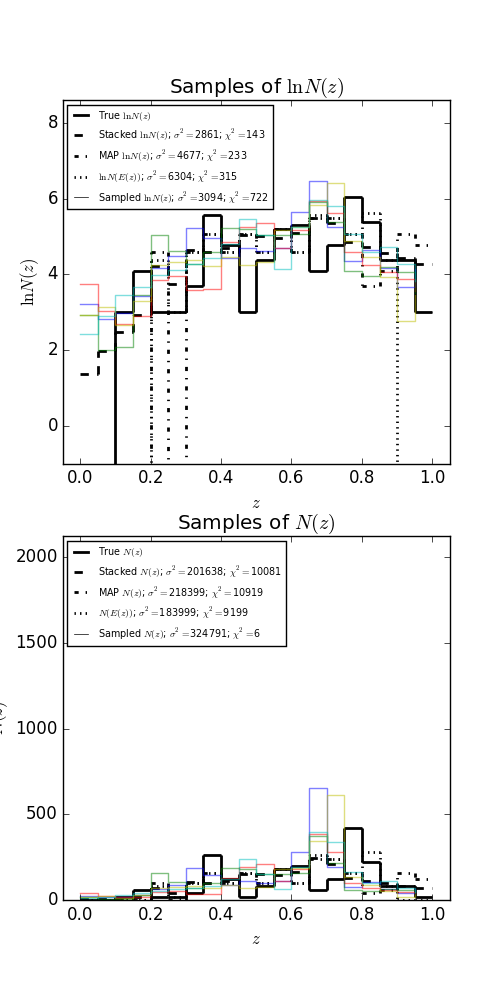
\includegraphics[width=0.5\textwidth]{sigma/samps.png}
%\caption{}
%\label{fig:noisyparam}
%\end{figure}

\clearpage
\subsection{Multimodal zPDFs}
\label{sec:multi}

In this test, we aim to simulate more realistic interim redshift posteriors by 
modifying the procedure of Sec. \ref{sec:mock} to introduce inaccuracy that 
causes catastrophic photo-z errors.  Catastrophic photometric redshift errors 
arise from a degeneracy in the space of galaxy SEDs and redshifts, wherein a 
galaxy of one type at one redshift has photometry indistinguishable from a 
galaxy of another type at another redshift.  To simulate this case, multimodal 
interim redshift posteriors will be considered.

In this case we introduce one change in Sec. \ref{sec:mock}.  Here, the 
redshift posteriors are sums of Gaussians of the form of those tested in Sec. 
\ref{sec:noisy}.  Each galaxy is assigned a number $R_{j}$ of Gaussian elements 
to be summed, chosen randomly from $1,\dots,K$ where $K$ is the dimensionality 
of $\vec{\theta}$.  The true redshift of each galaxy $z_{j}^{0}$ is used to 
generate to $R_{j}$ Gaussian elements with means 
$\{\{z_{j}^{r_{j}}\}_{R_{j}}\}_{J}$ and standard deviations 
$\{\{v_{j}'^{r_{j}}\}_{R_{j}}\}_{J}$.  Some examples of the multimodal zPDFs 
are shown in Fig. \ref{fig:multipzs}.  The rest of the procedure of Sec. 
\ref{sec:mcmc} is followed precisely.

\begin{figure}
%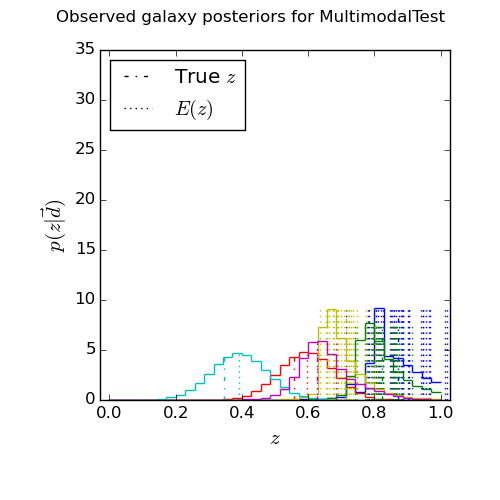
\includegraphics[width=0.5\textwidth]{multi/samplepzs.png}
\caption{}
\label{fig:multipzs}
\end{figure}

%\begin{figure}
%\includegraphics[width=0.5\textwidth]{multi/samps.png}
%\caption{}
%\label{fig:multiparam}
%\end{figure}

\clearpage
\subsection{Toy Model $N(z)$}
\label{sec:fake}

We test the sampler in a case of a highly unrealistic but strongly featured 
true $N(z)$.  This is done to show that the sampler works even in extreme and 
unanticipated conditions.  Here we modify the procedure of Sec. \ref{sec:mock}. 
 Instead of sampling the true distribution $p(z|\vec{\theta}')$, we sample a 
narrow Gaussian.  The rest of Sec. \ref{sec:mock} is followed precisely.  Sec. 
\ref{sec:mcmc} is followed without alteration.

\begin{figure}
%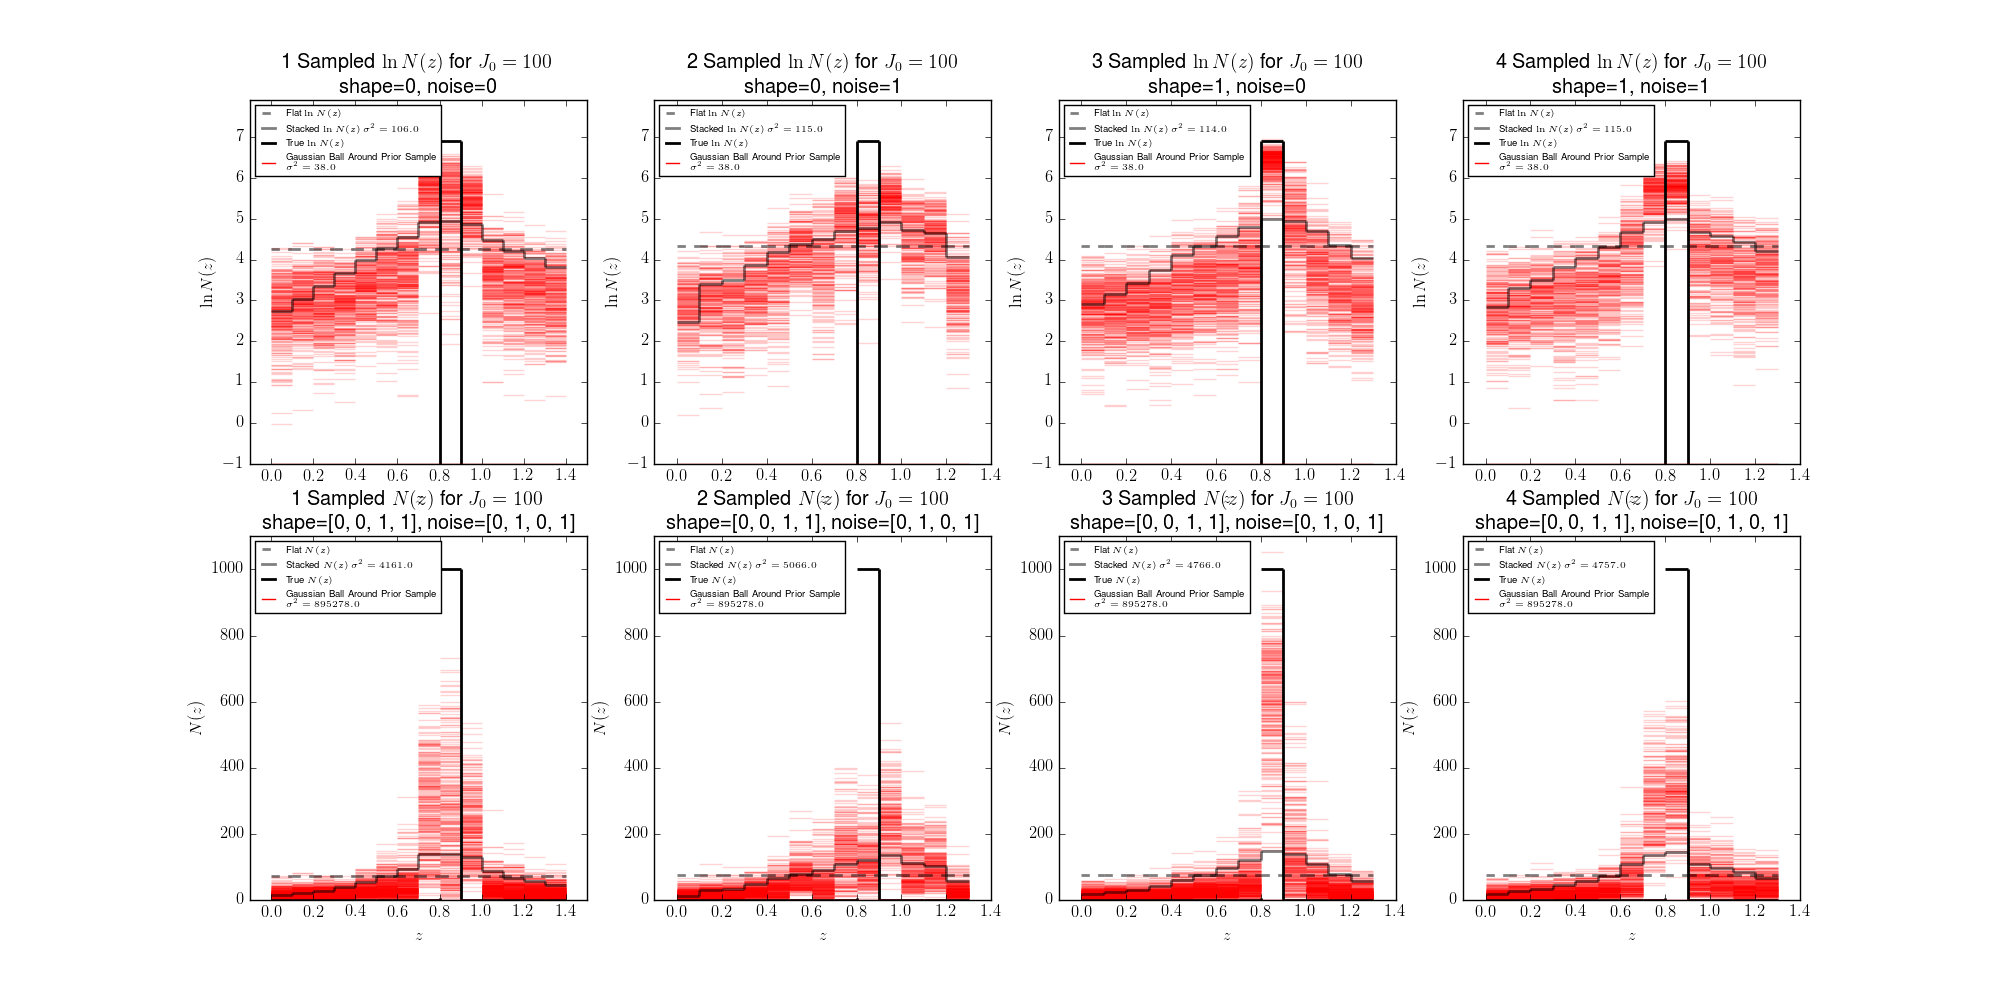
\includegraphics[width=0.5\textwidth]{samps-toy.png}
\caption{}
\label{fig:dumbestparam}
\end{figure}

\clearpage
\subsection{Variable Interim Prior}
\label{sec:interim}

In this case, we vary the interim prior used in Sec. \ref{sec:mock} to show 
that an appropriate choice of interim prior is crucial to sampler performance.  
Typically, interim redshift posteriors are made with an interim prior derived 
from $N(z)$ in a previous observational study.  Since most observational 
studies used for this purpose are spectroscopically confirmed and objects for 
which photometric redshifts are relied upon make up a population that cannot be 
spectroscopically confirmed, such an interim prior is rarely appropriate.  Some 
efforts have been made to modify an observationally informed interim prior so 
that it is more representative of the data set.  \citep{Sheldon2012}  However, 
any interim prior of this kind imparts information into the interim redshift 
posteriors.  Ideally, an uninformative interim prior would be used, although it 
may be complicated to compute from the covariances of the raw data.  In this 
test, we consider two obviously inappropriate interim priors and compare it to 
the flat interim prior used in previous tests according to Sec. \ref{sec:mock}. 
 The rest of the procedure of \ref{sec:mcmc} is followed precisely.

\clearpage
\subsection{Low-z Favoring Interim Prior}
\label{sec:lowz}

In some cases, the interim prior is determined directly from a previous 
spectroscopic redshift survey.  Because low-redshift galaxies are more likely 
to be bright enough to be observed by such a survey, $N(z)$ determined from 
that sample will be heavily biased to low redshift galaxies.  By contrast, the 
galaxies that were unobserved in such a survey are more likely be dimmer, 
making them more likely to be at higher redshifts.  Since the interim prior is 
not compatible with our beliefs about the true redshift distribution, the 
resulting interim redshift posteriors will be inappropriate.  In this test, we 
choose an interim prior with most of its weight at low redshifts.  The results 
of the inference are shown in Fig. \ref{fig:uparam}.

\begin{figure}
%\includegraphics[width=0.5\textwidth]{int-u/samps.png}
\caption{}
\label{fig:uparam}
\end{figure}

\clearpage
\subsection{Mid-z Disfavoring Interim Prior}
\label{sec:midz}

One potential method for selecting an interim prior with support over the 
entire redshift range expected of the photometric survey is to sum two or more 
$N(z)$ distributions obtained from reliable photometric surveys in the past.  
This is also problematic because the sum of redshift distributions for two or 
more surveys does not reflect our beliefs about the true distribution for a 
single survey.  To simulate this, we choose an interim prior with more weight 
at high and low redshifts than for mid-range redshifts.  The results of the 
inference are shown in Fig. \ref{fig:bparam}.

\begin{figure}
%\includegraphics[width=0.5\textwidth]{int-b/samps.png}
\caption{}
\label{fig:bparam}
\end{figure}

\clearpage
\section{Real Test}
\label{sec:boss}

In addition to simulated tests, we also apply this method to data described in 
Sec. \ref{sec:data}.  The results of the inference are shown in Fig. 
\ref{fig:dataparam}.

\begin{figure}
%\includegraphics[width=0.5\textwidth]{data/samps.png}
\caption{}
\label{fig:dataparam}
\end{figure}

\clearpage
\section{Discussion}
\label{sec:disc}

This study demonstrates a mathematically consistent implementation of inference 
of a one-point statistic based on zPDFs.  This work supports the production of 
zPDFs by upcoming photometric surveys such as LSST so that more accurate 
inference of physical parameters may be accessible to the scientific community. 
 We discourage researchers from co-adding zPDFs or converting them into point 
estimates of redshift and instead recommend the use of Bayesian probability to 
guide the usage of zPDFs in science.

The method herein developed is applicable with minimal modification to other 
one-point statistics of redshift to which we will apply this method in the 
future.  Such statistics include the redshift-dependent luminosity function and 
weak lensing mean distance ratio, the former of which is presented below in 
Sec. \ref{sec:lf}.

\clearpage
\subsection{The Luminosity Function}
\label{sec:lf}

Since the redshift-dependent luminosity function $\Phi(\vec{L},z)$ is a number 
density over redshift $z$ and one other parameter, luminosity $\vec{L}$ (which 
may be a vector if not bolometric), that contributes to the same data 
$\{\vec{d}_{j}\}_{J}$ in the form of a vector of photometric magnitudes, it is 
essentially a generalization of the redshift distribution function $N(z)$ 
previously investigated here; in other words, $N(z)$ is related to 
$\Phi(\vec{L},z)$ by way of an integral over luminosity.   We may express this 
as Eq. \ref{eq:lf}, where $\Phi(\vec{L},z)$ is parametrized by hyperparameters 
that are components of $\vec{\phi}$ .

\begin{eqnarray}
\label{eq:lf}
p(z_{j},\vec{L}_{j}|\vec{\phi}) &=& \frac{\Phi(\vec{L},z)}{\iint 
\Phi(\vec{L},z)\ d\vec{L}\ dz} = \frac{\Phi(\vec{L},z)}{\int N(z)\ dz} = 
\frac{1}{J}\ \Phi(\vec{L},z)
\end{eqnarray}

A graphical model for this problem is presented in Fig. \ref{fig:lf}.  As in 
Sec. \ref{sec:meth}, we shall outline the translation of this graphical 
representation of the probabilistic model using the same formalism.

\begin{figure}
\vspace{0.5cm}
\begin{center}
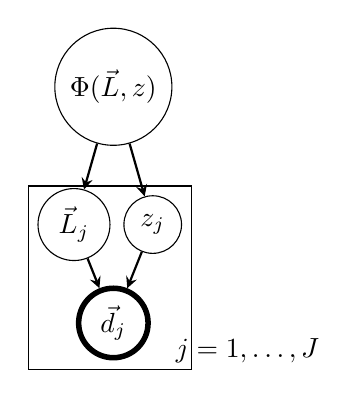
\begin{tikzpicture}[node distance=1cm]

\node (lf) [hyper] {$\Phi(\vec{L},z)$};
\node (z) [param, below of=lf,yshift=-0.75cm,xshift=0.5cm] {$z_{j}$};
\node (L) [param, below of=lf,yshift=-0.75cm,xshift=-0.5cm] {$\vec{L}_{j}$};
\node (flux) [data, below of=lf,yshift=-2cm] {$\vec{d}_{j}$};
\node (survey) [draw=black,fit={(L.west)(z.north)(flux.south)(z.east)}] {};
\node [xshift=1.75cm,yshift=0.25cm] at (survey.south) {$j=1,\dots,J$};

\draw [arrow] (lf) -- (z);
\draw [arrow] (lf) -- (L);
\draw [arrow] (z) -- (flux);
\draw [arrow] (L) -- (flux);

\end{tikzpicture}
\caption{This directed acyclic graph illustrates a hierarchical model for the 
luminosity function $\Phi(\vec{L},z)$.}
\label{fig:lf}
\end{center}
\end{figure}

First, we assume independence of the $J$ data points $\vec{d}_{j}$ where $J$ is 
a Poisson random variable with expected value $J_{0}$.  However, we acknowledge 
that the measurements are not independent if they are made as part of the same 
experimental design with shared equipment, not to mention the fact that 
$\vec{L}_{j}$ and $z_{j}$ are not independent of $\vec{L}_{j'\neq j}$ and 
$z_{j'\neq j}$ respectively due to the physics summarized by the luminosity 
function $\Phi(\vec{L},z)$.  However, given the assumption of independence, we 
may write the full likelihood as Eq. \ref{eq:lfind}.  

\begin{eqnarray}
\label{eq:lfind}
p(\{\vec{d}_{j}\}_{J}|\vec{\phi}) &=& e^{-\iint \Phi(\vec{L},z)\ dL\ dz}\ 
\prod_{j=1}^{J}\ p(\vec{d}_{j}|\vec{\phi})
\end{eqnarray}

As before, we apply Bayes' Rule to relate the full likelihood to the full 
posterior in Eq. \ref{eq:lfbayes} and expand out the individual likelihood in 
terms of the parameters $\{\vec{L}_{j}\}_{J}$ and $\{z_{j}\}_{J}$ in Eq. 
\ref{eq:lfexpand}.

\begin{eqnarray}
\label{eq:lfbayes}
p(\vec{\phi}|\{\vec{d}_{j}\}_{J}) &=& 
\frac{p(\vec{\phi})}{p(\{\vec{d}_{j}\}_{J})}e^{-\iint \Phi(\vec{L},z)\ 
d\vec{L}\ dz}\ \prod_{j=1}^{J}\ p(\vec{d}_{j}|\vec{\phi})
\end{eqnarray}

\begin{eqnarray}
\label{eq:lfexpand}
p(\vec{\phi}|\{\vec{d}_{j}\}_{J}) &=& 
\frac{p(\vec{\phi})}{p(\{\vec{d}_{j}\}_{J})}e^{-\iint \Phi(\vec{L},z)\ 
d\vec{L}\ dz}\ \prod_{j=1}^{J}\ \iint\ p(\vec{d}_{j}|z_{j},\vec{L}_{j})\ 
p(z_{j},\vec{L}_{j}|\vec{\phi}) dz_{j}\ d\vec{L}_{j}
\end{eqnarray}

If we are unable to access the individual likelihoods, as is in general the 
case, we will repeat the trick of using an interim prior value of 
hyperparameters $\vec{\phi}^{0}$.  This results in Eq. \ref{eq:lftrick}.

\begin{eqnarray}
\label{eq:lftrick}
p(\vec{\phi}|\{\vec{d}_{j}\}_{J}) &=& 
\frac{p(\vec{\phi})}{p(\{\vec{d}_{j}\}_{J})}e^{-\iint \Phi(\vec{L},z)\ 
d\vec{L}\ dz}\ \prod_{j=1}^{J}\ \iint\ 
p(z_{j},\vec{L}_{j}|\vec{d}_{j},\vec{\phi}^{0})\ 
\frac{p(z_{j},\vec{L}_{j}|\vec{\phi})}{p(z_{j},\vec{L}_{j}|\vec{\phi}^{0})} 
dz_{j}\ d\vec{L}_{j}
\end{eqnarray}

%Fig. \ref{fig:sheldon} compares the result of summing the posteriors as in Eq. 
\ref{eq:sheldon} with the result of the MCMC solutions of Eq. \ref{eq:bayes}.  
The method of \citet{Sheldon2012} underestimates the probability of observing 
low redshifts.  As one would expect, the MCMC estimate irreversibly loses some 
substructure because of the shifting error added to the simulated data.

%\begin{figure}
%\label{fig:sheldon}
%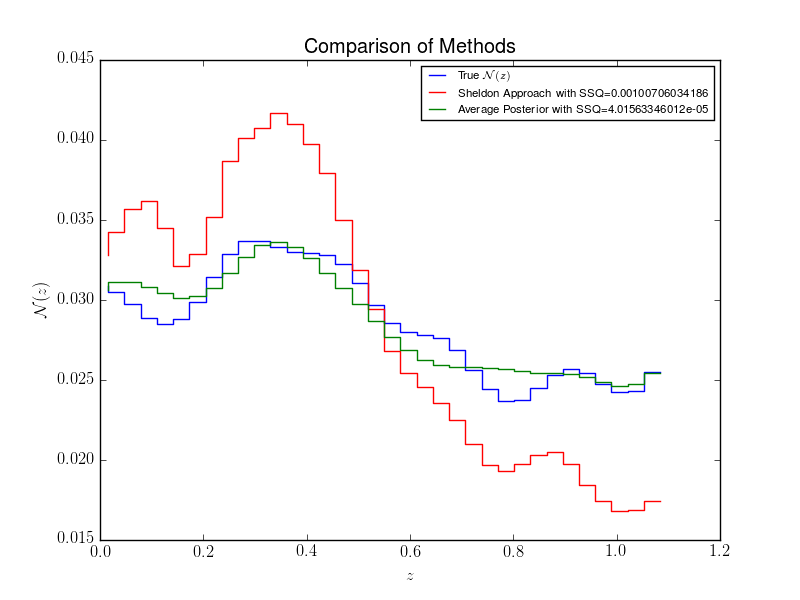
\includegraphics[width=\textwidth]{compare-sheldon.png}
%\caption{The result of applying Eq. \ref{eq:sheldon} is shown in red, the 
average accepted posterior sample from the method presented here is shown in 
blue, and $p(z)$ for the observable redshifts of Eq. \ref{eq:zshift} is shown 
in black.  The sum of squared differences between the result of each method and 
the true value are also shown; one can see that the \citet{Sheldon2012} 
approach has larger errors.}
%\end{figure}

%\acknowledgments

%\subsubsection{}
%\label{app:dumber}

%We next consider a set of $J$ galaxies representing a draw from the Poisson 
distribution $P(J_{0},J_{0})$ for $J_{0}=100$.  The galaxies share a single 
true redshift $z^{s}$ arbitrarily chosen to be the midpoint of the redshift bin 
with the largest $\theta_{k}$.  The redshift posteriors are taken to be single 
Gaussians centered at observed redshifts $z^{p}_{j}\sim 
N(z^{s},\bar{\Delta}(1+z^{s}))$ with shared variances of 
$\bar{\Delta}(1+z^{s})$. 

%\subsubsection{}
%\label{app:dumb}

%The last test case is comprised of a set of $J$ galaxies representing a draw 
from the Poisson distribution $P(J_{0},J_{0})$ for $J_{0}=1000$.  The true 
galaxy redshift bins $b_{j}=k$ from $k=1,\dots,K$ are assigned to each galaxy 
$j$ by randomly sampling the $K$ bins with weights given by the true redshift 
function of Eq. \ref{eq:truenz} as $\int_{z_{k}}^{z_{k+1}}p^{0}(z)dz$. True 
redshifts $z^{s}_{j}$ are assigned within these bins assuming a random uniform 
distribution within each bin.  The redshift posteriors are taken to be single 
Gaussians centered at observed redshifts $z^{p}_{j}\sim 
N(z^{s}_{j},\bar{\Delta}(1+z^{s}_{j}))$ with variances $\sigma_{j}\sim 
N(z^{s}_{j},\bar{\Delta}(1+z^{s}_{j}))$. 

\bibliographystyle{apj}
\bibliography{zPDF}

\end{document}